\section{Ion Thrusters}

\subsection{Operating Principles}

Ion thrusters are electrostatic devices that achieve high exhaust velocities by decoupling ionization from acceleration, entirely removing the thermodynamic limits of electrothermal systems. Operation occurs in three sequential stages: ionization, electrostatic acceleration, and beam neutralization. Inside a positively biased discharge chamber, a hollow cathode emits electrons that bombard neutral propellant (typically xenon) to form positive ions. These ions drift toward the ion optics—a highly positive screen grid and a negative accelerator grid—which extract and axially accelerate the beam \cite{fep_book}. Finally, a downstream neutralizer cathode injects electrons into the exhaust to prevent spacecraft charging \cite{holste_2020}. 

\begin{figure}[htb]
    \centering
    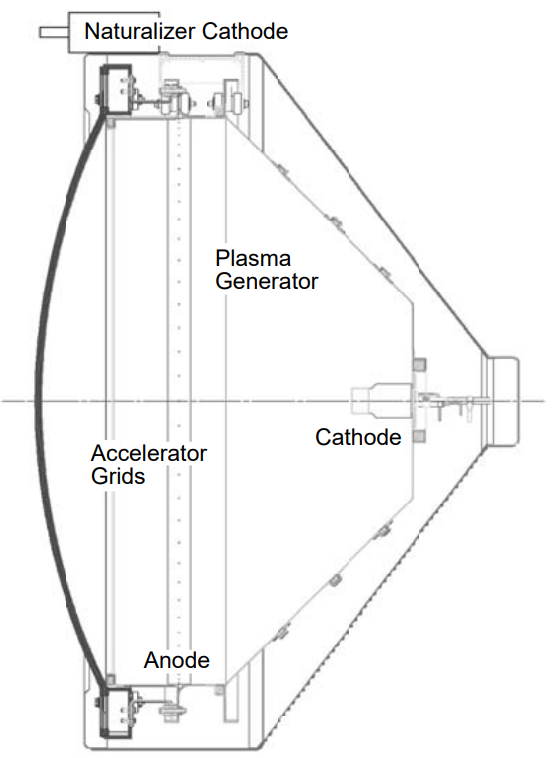
\includegraphics[width=0.25\textwidth]{figs/ion_thrusters_1.png}
    \caption{Cross-section of a gridded ion thruster (electron bombardment type) \cite{fep_book}}
    \label{fig:git_schematic}
\end{figure}

%A notable variant is the radio-frequency ion thruster (RIT), which replaces the internal cathode with an RF coil for inductive plasma heating, thereby eliminating cathode erosion and extending lifespan \cite{holste_2020}.

\subsection{Propellant Selection}

Propellant selection balances high atomic mass, low ionization energy, chemical inertness, and storability \cite{dietz_2019}. Xenon (131.3~amu, 12.13~eV) offers the best compromise and remains the industry standard \cite{fep_book, dietz_2019}. Krypton is increasingly used in commercial constellations (e.g., Starlink) to reduce costs, despite requiring higher jet power for equivalent thrust \cite{holste_2020}. Legacy propellants like cesium and mercury are obsolete due to toxicity and spacecraft contamination.

\begin{table}[htb]
\centering
\caption{Properties of selected ion thruster propellant candidates \cite{dietz_2019, fep_book}}
\label{tab:ion_propellants}
\begin{tabular}{@{}llll@{}}
\toprule
\textbf{Propellant} & \textbf{Atomic/Mol.} & \textbf{1st Ionization} & \textbf{Status} \\
                    & \textbf{Mass (amu)}  & \textbf{Energy (eV)}    &                 \\ \midrule
Xenon (Xe)   & 131.3 & 12.13 & Industry standard \\
Krypton (Kr) & 83.8  & 14.00 & Commercial (Starlink) \\
Iodine (I)   & 126.9 & 10.45 & Research / CubeSat \\
Cesium (Cs)  & 132.9 & 3.89  & Obsolete (toxic) \\
Indium (In)  & 114.8 & 5.79  & FEEP micro-thrusters \\ \bottomrule
\end{tabular}
\end{table}

\subsection{Performance Equations}

\subsubsection{Exhaust Velocity \& Thrust}

An ion of charge $q$ and mass $M$ accelerated through a net potential difference $V_b$ gains kinetic energy, defining the exhaust velocity \cite{holste_2020}:

\begin{equation}
\label{eq:ion_ve}
    v_e = \sqrt{\frac{2 q V_b}{M}}
\end{equation}

where $q = e = 1.602 \times 10^{-19}$~C for singly charged ions. Thrust is the momentum flux of the accelerated beam \cite{fep_book}:

\begin{equation}
\label{eq:ion_thrust}
    T = \dot{m} \, v_e = I_b \sqrt{\frac{2 M V_b}{q}}
\end{equation}

While inherently low-thrust (e.g., NSTAR produces 20--90~mN at 2.3~kW), continuous operation over months accumulates massive $\Delta v$ with minimal propellant \cite{holste_2020}.

\subsubsection{Specific Impulse}

Specific impulse ($I_{sp} = v_e/g_0$) routinely reaches 1500--10\,000~s in flight-qualified GIEs, far exceeding chemical limits \cite{holste_2020}. By the Tsiolkovsky equation:

\begin{equation}
\label{eq:tsiolkovsky}
    \Delta v = I_{sp} \, g_0 \ln\left(\frac{m_0}{m_f}\right)
\end{equation}

this high $I_{sp}$ yields exceptionally favorable mass ratios. For $\Delta v > 5$~km/s, chemical propulsion becomes practically infeasible, making ion propulsion an enabling technology \cite{holste_2020}.

\subsubsection{Efficiency Metrics}

Thruster performance is primarily characterized by mass utilization ($\eta_m$) and overall thruster efficiency ($\eta_T$). \textbf{Mass utilization efficiency} captures the fraction of admitted propellant that is ionized and accelerated \cite{holste_2020}:

\begin{equation}
\label{eq:ion_massutil}
    \eta_m = \frac{\dot{m}_i}{\dot{m}_p} = \frac{I_b M}{e \dot{m}_p}
\end{equation}

\textbf{Thruster efficiency} is the ratio of jet power to total electrical input power ($P_{in}$) \cite{holste_2020, fep_book}, which expands directly into its constituent sub-efficiencies:

\begin{equation}
\label{eq:ion_eff}
    \eta_T = \frac{T^2}{2 \dot{m}_p P_{in}} = \eta_e \eta_m \xi^2
\end{equation}

where $\eta_e$ is the \textbf{electrical efficiency} (fraction of input power successfully converted to beam power) and $\xi$ is the \textbf{thrust correction factor} accounting for beam divergence and multiply-charged ions. %A key secondary metric is the \textbf{ion production cost} $\eta_d = P_d / I_b$, representing the discharge power spent per ion \cite{holste_2020}. For GIEs, this amounts to several hundred eV---well above xenon's ionization threshold---constituting the dominant internal loss mechanism.

\subsection{Specific Characteristics and Limitations}

Grid erosion from charge-exchange (CEX) collisions is the primary wear mechanism, limiting operational lifetime to roughly 10,000--100,000 hours. During CEX, fast extracted ions interact with neutral propellant to create slow secondary ions that are drawn back to sputter the negatively biased accelerator grid \cite{holste_2020}. Operationally, thrusters are heavily constrained by electrical power; inverse-square solar power losses eventually necessitate nuclear sources for deep-space missions. Furthermore, the supply of xenon—a rare byproduct of air liquefaction—is a growing bottleneck. Rising prices driven by mega-constellations have rapidly accelerated research into cheaper alternatives like krypton and iodine \cite{holste_2020, dietz_2019}.

%\begin{table}[htb]
%\centering
%\caption{Typical performance parameters of gridded ion thrusters \cite{holste_2020, fep_book}}
%\label{tab:ion_performance}
%\begin{tabular}{@{}ll@{}}
%\toprule
%\textbf{Parameter} & \textbf{Typical Value} \\ \midrule
%Thrust Range             & 0.01~mN -- 750~mN \\
%Specific Impulse         & 1\,500 -- 10\,000~s \\
%Exhaust Velocity         & 15 -- 100~km/s \\
%Thruster Efficiency      & 30 -- 90\% \\
%Thrust-to-Power Ratio    & 20 -- 250~mN/kW \\
%Input Power              & 0.1 -- 20~kW \\
%Typical Propellants      & Xe, Kr, I$_2$ \\
%Operational Lifetime     & Years \\ \bottomrule
%\end{tabular}
%\end{table}